\section{ИССЛЕДОВАНИЕ РАБОТЫ ДЕШИФРАТОРА}

\begin{figure}[H]
	\centering
	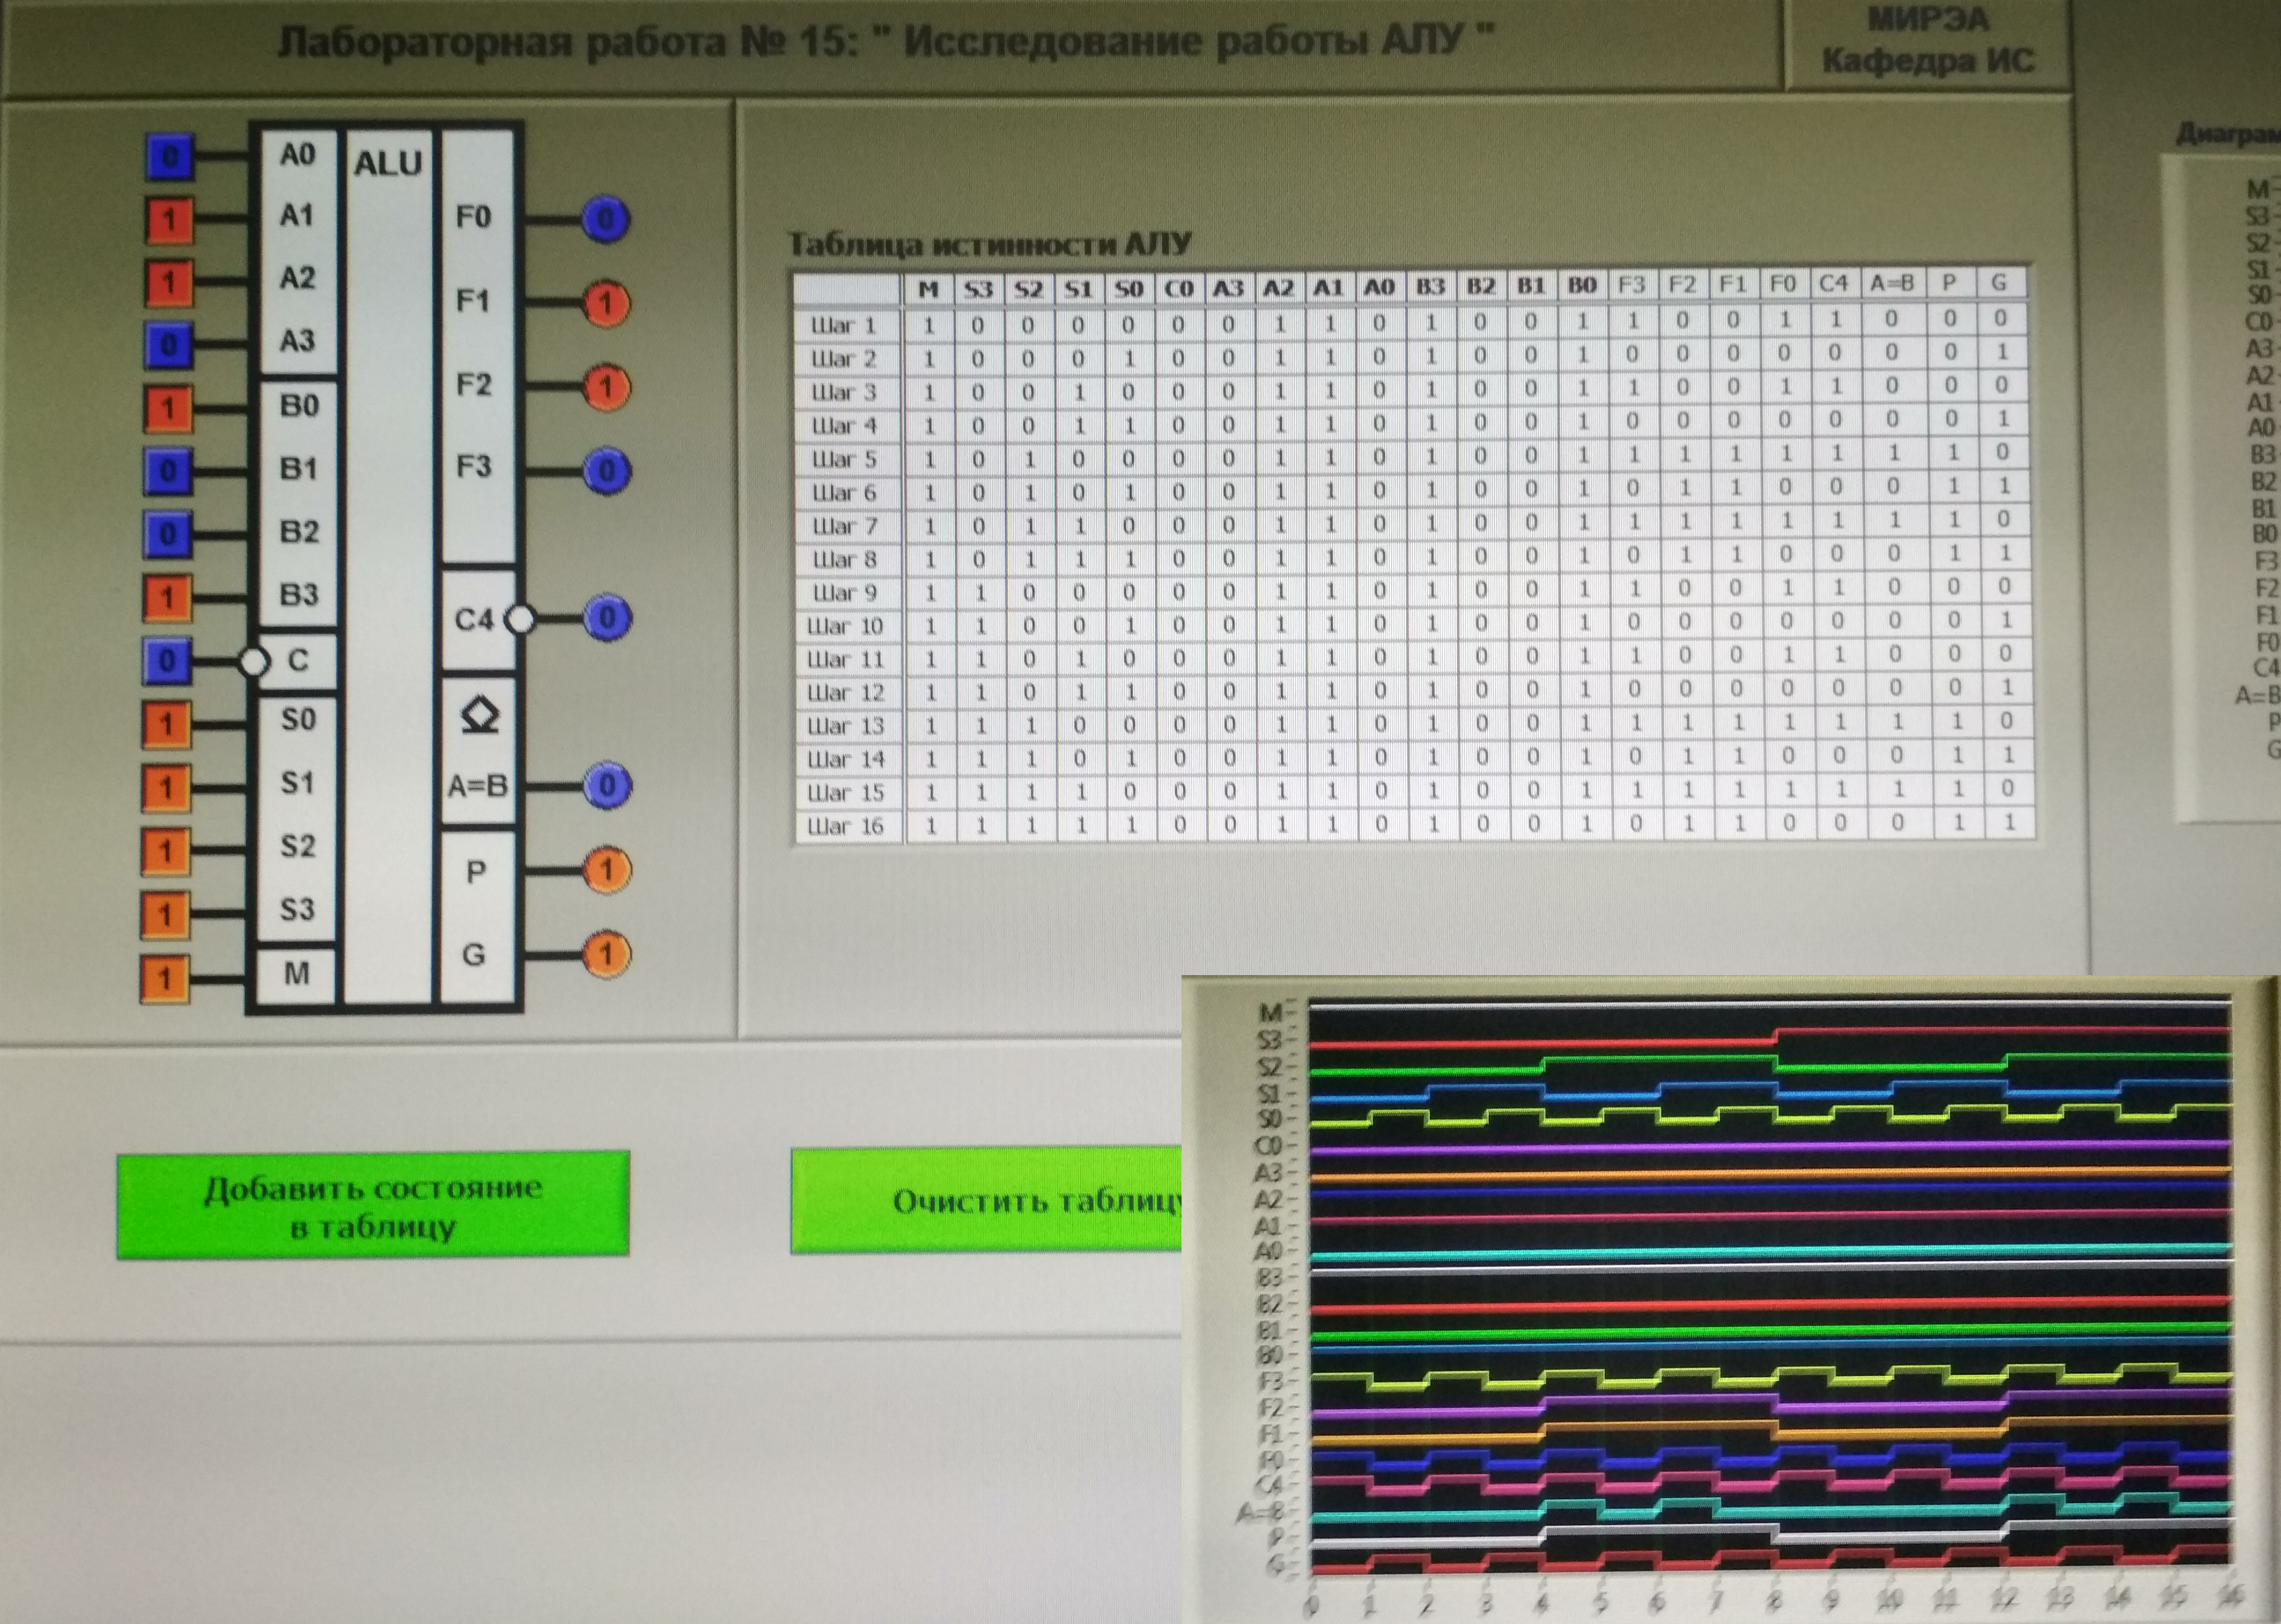
\includegraphics[width=0.95\linewidth]{imgs/3/1}
	\caption{Результат работы дешифратора}
	\label{fig:3_}
\end{figure}

В ходе работы было выяснено, что для работы дешифратора необходимо подать низкий уровень на вход E.
% Шифратор является приоритетным, вход X6 имеет больший приоритет, чем X3

Элемент SN74LV138AT

Характеристики:
\begin{itemize}
	\item 3-Line To 8-Line Decoder
	\item Typical data delay 7.6 ns at 5 V
	\item 4.5V to 5.5V $V_{CC}$ Operation
	\item Low voltage TTL family
\end{itemize}